\section*{\hypertarget{gm}{Game Master}}
"Tough...Don't blame us. Blame yourself or God."\\
\indent -- Delita

\begin{center} 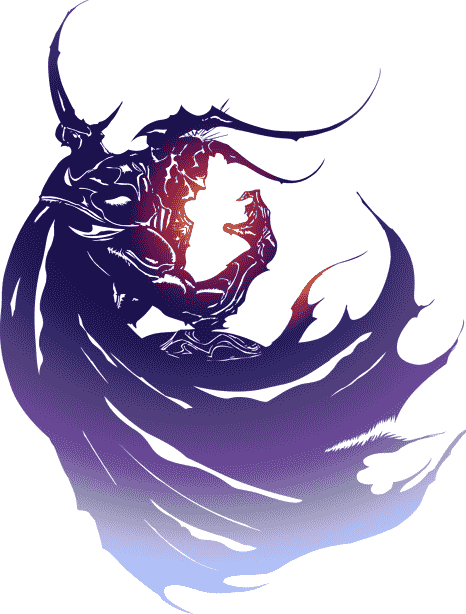
\includegraphics[width=\columnwidth]{./art/images/ff4.png} \end{center}
%
\addcontentsline{toc}{section}{Game Master}
%
The Game Master has a different role compared to the players, who play from the perspective of the protagonists.
He creates the world and setting of the adventure and takes the role of all non-player characters.
Furthermore, the GM describes the environment and narrates the outcomes of all actions. 
This section provides guidelines, that help GMs to get a better understanding of their role.
Moreover, it includes a variety of content that you can use to create your game world.

\subsubsection*{Sessions}
Most adventures are too long to be completed in a single sitting, so they have to be divided into multiple sessions.
Therefore, it is sufficient to prepare content only for the next session instead of everything in advance.
During gameplay, look out for opportunities to gracefully end an ongoing session, e.g. after conclusion of a quest.
Sessions can be planned according to adventure \hyperlink{ms}{Milestones}, where Level ups should occur roughly every 1-3 sessions.
Still, you will not be able to prepare for everything, so do not be afraid to improvise when necessary.

\pagebreak

\subsubsection*{Using Checks}
Checks are a powerful tool that help you decide the outcome of uncertain actions.
When players attempt actions you can ask them for checks by assigning a secret DC to the task.
In some situations you can also proactively ask players to make checks, e.g. to decide whether the party notices an ambush.
All non-player characters controlled by you may also have to do checks, as they follow the same rules.
However, you do not have to use checks if the outcome of an action is reasonably clear.  

\subsubsection*{Combat}
During combat, you play the role of all non-player characters and all \hyperlink{combat}{Combat Rules} apply to them. 
Unlike the players, you may keep most information secret, such as remaining HP \& MP and dice rolls.
While playing as an enemy group, you should make decisions from their perspective without using your own knowledge.
When creating combat encounters, aim to balance out the number of participants on both sides.
Large hordes of weaker monsters will often overwhelm the party, while a lone strong enemy might not stand a chance.
A healthy mix of different enemies makes combat more interesting and balanced.
In addition, it also helps to use visual aids like maps to keep track of the battlefield.
Battles are a matter of life and death, so they usually take up a significant portion of playtime.
Therefore, try to keep the focus on the important battles of the adventure.   

\subsubsection*{Narrating \& Roleplaying}
To immerse yourself and the players into your world, it is helpful to give short, vivid descriptions of the party's current surroundings.
In doing this, focus on elements that could be interesting for the players to interact with.
Likewise, picture the descriptions given by players about their character's actions to create your narrations of the outcome.
This often requires you to take the role of many different characters yourself to interact with the party.
In that case, try to understand the perspective of the character to portray how they would talk and act when confronted with the party.

\vspace{1cm} 

\example{Using Checks}{
Zidane and Blank try to deliver a convincing staged sword fight to an audience of nobles.
The GM decides that this is a difficult task (DC 9), because the nobles have high expectations. 
Zidane rolls 2d with the result 9, so he barely passes the check. 
Accordingly, the GM decides that most of the nobles are happy with the delivered performance. 
Queen Brahme however, is not impressed. 
}

\pagebreak

\subsubsection*{Travel \& Time}
The players can get familiar with the world, by exploring many different locations.
However, travelling on foot is often not the best choice due to difficult terrain, weather or ambushes.
Depending on the setting, more comfortable transportation might be available such as ships, trains, airships, cars or \hyperlink{chocobo}{Chocobos}.
Usually, the party needs to employ such a service, but as they become more wealthy, they may acquire their own vehicles.
For longer journeys, try to keep track of the amount that passes, which also affects the rest of the world.
In general, time passes at a different speed in the game than at your table.
This is because uneventful aspects of the adventure can be narrated quickly, while important decisions need to be thought through more carefully.

\subsubsection*{Wealth}
You can give players incentives to complete certain tasks by rewarding Gil, Items and Equipment.  
By default, these earned rewards should be evenly divided between all party members.
Another way for players to accumulate more wealth is by trading with non-player characters. 
Generally, merchants try to sell wares above their original value and buy them at no more than half their original value to stay profitable. 
In addition, you can consider modifying the cost of resting in Inns or Tents to adjust the game difficulty.

\vspace{1.2cm}

\example{Narrating \& Roleplaying}
{
	\begin{description}[leftmargin=*]
		\item[Yasumi (Game Master):]
		As you enter Riovannes Castle, you find yourself inside a large hall with narrow water streams running on both sides.
		Among multiple dead knights that lie scattered on the ground, you can see a man standing at the end of the central stairway.
		He turns around and you realize it is none other than Wiegraf Folles!			
		\item[Yasumi (playing as Wiegraf):] There you are Ram- \\ za. Draw your sword. 			
		\item[Akihiko:] I don't draw my sword yet. Maybe we can solve this peacefully.		
		\item[Yasumi (playing as Wiegraf):] What's wrong? If you don't, I will.			
		\item[Akihiko (playing as Ramza):] How miserable you are. Giving away your spirit just to avenge yourself.
		\item[Yasumi (playing as Wiegraf):] Revenge? That's not what I'm after. 
		I want to bring chaos into the world... But, don't worry. I'll kill you myself!			
		\item[Akihiko:] OK, NOW I definitely draw my sword!
		\item[Yasumi:] Alright, let's roll initiative then.
	\end{description}
}

\pagebreak

\subsubsection*{Side Quests}
While the adventure should generally strive towards solving the central conflict, an occasional digressing session can be helpful to relieve tension.
The list on below shows some ideas for such short side plots.
\begin{description}[leftmargin=*]
	
	\item[\color{accent} Casino:]
	The party finds an extravagant Casino, which offers various gambling games.
	Although it does not look like it at first, you will never find a more wretched hive of scum and villainy.
	If the party wants to play a game, you can use very hard checks to decide the outcome.
	However, all games are rigged against the players, so making a profit here is almost impossible.
	
	\item[\color{accent} Chocobo Farm:]
	The party finds a \hyperlink{chocobo}{Chocobo} farm. 
	The farmer is nice and apologizes for not being able to rent out his Chocobos currently. 
	He mentions that recently some of them have been disappearing at night and he is desperate to resolve the mystery.
	If the party finds the cause for their disappearance, the farmer shows his gratitude by lending his Chocobos to them for free.
	
	\item[\color{accent} Coliseum:]
	The party finds the Coliseum, an arena where adventurers fight monsters and other adventurers for entertainment.
	The owner of the establishment offers generous rewards to the party for participating.
	If they accept, the party has to fight multiple consecutive battles where failure means certain death.
	Also, most of the viewers place bets on the fighters, which the party can try to use to their advantage.
	
	\item[\color{accent} Master Craftsman:]
	The party finds a workshop run by a man named Cid.
	Cid is a master craftsman, he can for example be a mechanic or a smith.
	He complains to the party about not being able to work, because he is not getting any material deliveries.
	He offers his services to them as a reward if they manage to bring him a set of rare materials.
	
	\item[\color{accent}Mystery Cave:]
	The party meets two soldiers named Biggs and Wedge.
	The two were tasked with finding a group of researchers who have gone missing in a cave nearby.
	They seem very scared, so they offer the party half of the reward for their help. 
	They seem to know more about this incident than they are letting on.
	
	\item[\color{accent} Zone Eater:]
	The party gets surprised by a much larger version of the \hyperlink{abyssworm}{Sand Worm} called "Zone Eater".
	Despite any effort, the party gets inhaled by the beast and the adventurers find themselves inside its apparently endless stomach.
	They quickly realize that they are not the first to suffer this fate, as many monsters, treasures and even other people are stuck with them.
\end{description}
\pagebreak
